\documentclass[12pt,a4paper]{article}
\usepackage[utf8]{inputenc}
\usepackage[T5,T1]{fontenc}
\usepackage[english]{babel}
\usepackage{graphicx}
\usepackage{listings}
\usepackage{xcolor}
\usepackage{xurl}
\usepackage{hyperref}
\usepackage{geometry}
\usepackage{amsmath}
\usepackage{amssymb}
\usepackage{booktabs}
\usepackage{tikz}
\usetikzlibrary{shapes.geometric, arrows, positioning, trees}

\geometry{margin=1in}
\setlength{\emergencystretch}{3em}

\definecolor{codegreen}{rgb}{0,0.6,0}
\definecolor{codegray}{rgb}{0.5,0.5,0.5}
\definecolor{codepurple}{rgb}{0.58,0,0.82}
\definecolor{backcolour}{rgb}{0.96,0.96,0.93}

\lstdefinestyle{mystyle}{
    backgroundcolor=\color{backcolour},   
    commentstyle=\color{codegreen},
    keywordstyle=\color{magenta},
    numberstyle=\tiny\color{codegray},
    stringstyle=\color{codepurple},
    basicstyle=\ttfamily\footnotesize,
    breakatwhitespace=false,         
    breaklines=true,                 
    captionpos=b,                    
    keepspaces=true,                 
    numbers=left,                    
    numbersep=5pt,                  
    showspaces=false,                
    showstringspaces=false,
    showtabs=false,                  
    tabsize=2,
    language=C++
}

\lstset{style={mystyle}}

\title{\textbf{CS202 Design Pattern Report: Mediator Pattern}\\\large Centralized Airspace Traffic Coordination, $O(N^2)$ Mesh Decoupling, and Modern C++17 Architecture}
\author{\textbf{Group 52} \\ {\fontencoding{T5}\selectfont Nguyễn Đình Minh Huy} (Student ID: 25125083) \\ {\fontencoding{T5}\selectfont Trần Gia Huy} (Student ID: 25125084)}
\date{\today}

\begin{document}

\maketitle
\tableofcontents
\newpage

\section{Real-world Problem \& Motivation}

\subsection{Background: Airport Airspace and Runway Coordination}
In modern aviation and distributed software systems, coordinating multiple independent, concurrent entities that contend for shared, safety-critical resources is a central architectural challenge. Consider an international airport managing active airspace within a terminal radar service area. Multiple types of aircraft operate simultaneously:
\begin{itemize}
    \item \textbf{Commercial Passenger Jets (e.g., VN123, BA789):} Carrying hundreds of passengers on fixed flight schedules.
    \item \textbf{Heavy Cargo Transports (e.g., FX902):} Operating freight logistics with specific runway weight allowances.
    \item \textbf{Emergency Air Ambulances / Medevac (e.g., MEDIC1):} Transporting critical patients with low fuel reserves, requiring immediate priority runway clearance.
\end{itemize}

All aircraft must share a finite, exclusive physical resource: the active runway (\texttt{Runway 07L}). At most one aircraft may safely occupy the runway at any given instant for landing or takeoff.

\subsection{\texorpdfstring{The Communication Bottleneck: $O(N^2)$ Peer-to-Peer Mesh}{The Communication Bottleneck: O(N^2) Peer-to-Peer Mesh}}
If aircraft coordinate landing authorization directly with one another without a central coordinator (a peer-to-peer mesh architecture):
\begin{enumerate}
    \item \textbf{Complete Graph Complexity:} For $N$ active aircraft in the airspace, every aircraft must maintain direct radio and data links to all $N-1$ other aircraft. The total number of communication channels in the network forms a complete graph $K_N$ with:
    \begin{equation}
        E = \frac{N(N-1)}{2} = O(N^2)
    \end{equation}
    \item \textbf{High Entry/Exit Overhead:} When a new flight enters the airspace, it must establish $N$ new bidirectional links. When a flight touches down and exits the airspace, all remaining $N-1$ aircraft must execute cleanup routines.
    \item \textbf{Decentralized State Inconsistency and Deadlocks:} Because coordination logic is distributed across independent nodes, concurrent landing requests create race conditions, priority inversion, and potential mid-air collision hazards.
\end{enumerate}

\begin{figure}[htbp]
\centering
\resizebox{0.75\linewidth}{!}{
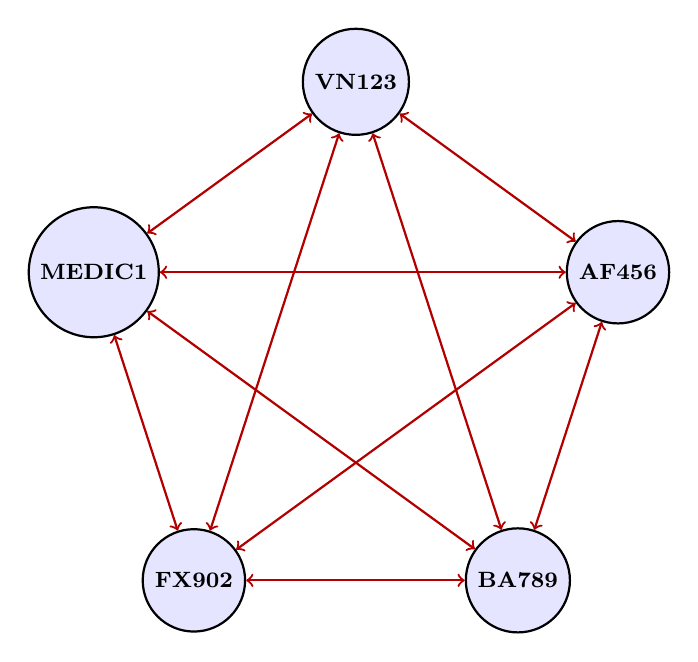
\begin{tikzpicture}[
    node/.style={circle, draw=black, thick, fill=blue!10, minimum size=1.3cm, font=\footnotesize\bfseries},
    conn/.style={<->, thick, red!70!black}
]
\node[node] (A) at (90:3.5cm) {VN123};
\node[node] (B) at (18:3.5cm) {AF456};
\node[node] (C) at (306:3.5cm) {BA789};
\node[node] (D) at (234:3.5cm) {FX902};
\node[node] (E) at (162:3.5cm) {MEDIC1};

\draw[conn] (A) -- (B);
\draw[conn] (A) -- (C);
\draw[conn] (A) -- (D);
\draw[conn] (A) -- (E);

\draw[conn] (B) -- (C);
\draw[conn] (B) -- (D);
\draw[conn] (B) -- (E);

\draw[conn] (C) -- (D);
\draw[conn] (C) -- (E);

\draw[conn] (D) -- (E);
\end{tikzpicture}
}
\caption{Decentralized Peer-to-Peer Flight Mesh with $O(N^2)$ Inter-Dependencies}
\label{fig:p2p_mesh}
\end{figure}

\subsection{Problem Statement}
The objective is to design a software architecture that enables aircraft to request landing authorization, handle holding patterns, receive runway vacancy cascades, and yield to emergency priority flights without aircraft having any compile-time or runtime knowledge of other individual aircraft instances.

\newpage
\section{Naive Solution}

In a naive object-oriented design without a mediator, aircraft maintain explicit pointer collections of all peer aircraft instances. Each aircraft executes a decentralized consensus loop before attempting to acquire the runway.

\begin{lstlisting}[caption={Naive Flight Coordination with Direct Peer Mesh (\texttt{naive.cpp})}]
namespace naive {

enum class FlightStatus {
    IN_FLIGHT,
    HOLDING_PATTERN,
    ON_RUNWAY,
    LANDED,
    PARKED_AT_GATE
};

enum class FlightType {
    COMMERCIAL,
    CARGO,
    EMERGENCY
};

class NaiveFlight {
private:
    std::string flightCode_;
    FlightType type_;
    FlightStatus status_;
    int capacityOrWeight_;
    
    // Tightly coupled: Every flight maintains direct pointers to all active peers (O(N^2) mesh)
    std::vector<NaiveFlight*> peerNetwork_;

public:
    NaiveFlight(std::string code, FlightType type, int capacityOrWeight)
        : flightCode_(std::move(code)),
          type_(type),
          status_(FlightStatus::IN_FLIGHT),
          capacityOrWeight_(capacityOrWeight) {}

    ~NaiveFlight() {
        leaveAirspaceNetwork();
    }

    void addPeer(NaiveFlight* peer) {
        if (peer != this && std::find(peerNetwork_.begin(), peerNetwork_.end(), peer) == peerNetwork_.end()) {
            peerNetwork_.push_back(peer);
        }
    }

    void removePeer(NaiveFlight* peer) {
        peerNetwork_.erase(
            std::remove(peerNetwork_.begin(), peerNetwork_.end(), peer),
            peerNetwork_.end()
        );
    }

    // Joins airspace: Wires this flight to all current flights, and all current flights to this flight
    void joinAirspaceNetwork(std::vector<NaiveFlight*>& currentAirspace) {
        for (auto* peer : currentAirspace) {
            this->addPeer(peer);
            peer->addPeer(this); // Bidirectional mutual registration
        }
        currentAirspace.push_back(this);
    }

    // Leaves airspace: Must notify and unhook from every peer
    void leaveAirspaceNetwork() {
        if (peerNetwork_.empty()) return;
        for (auto* peer : peerNetwork_) {
            peer->removePeer(this); // Mutate peer's internal collection
        }
        peerNetwork_.clear();
    }

    // Decentralized consensus algorithm: The flight polls all peers to determine if it is safe to land
    bool requestLandingPermission() {
        std::cout << "[" << flightCode_ << "] Requesting landing permission by polling "
                  << peerNetwork_.size() << " peers...\n";

        for (auto* peer : peerNetwork_) {
            // Check 1: Is any peer currently occupying the runway?
            if (peer->getStatus() == FlightStatus::ON_RUNWAY) {
                status_ = FlightStatus::HOLDING_PATTERN;
                std::cout << "  -> CONFLICT: Peer " << peer->getCode() 
                          << " is currently ON_RUNWAY. Entering HOLDING_PATTERN.\n";
                return false;
            }

            // Check 2: Does an emergency peer have priority?
            if (type_ != FlightType::EMERGENCY && peer->getType() == FlightType::EMERGENCY &&
                (peer->getStatus() == FlightStatus::HOLDING_PATTERN || peer->getStatus() == FlightStatus::IN_FLIGHT)) {
                status_ = FlightStatus::HOLDING_PATTERN;
                std::cout << "  -> PRIORITY YIELD: Emergency peer " << peer->getCode() 
                          << " has priority. Entering HOLDING_PATTERN.\n";
                return false;
            }
        }

        // Consensus reached
        status_ = FlightStatus::ON_RUNWAY;
        std::cout << "  -> CONSENSUS APPROVED: All peers report runway clear. Status: ON_RUNWAY.\n";
        return true;
    }

    void touchdown() {
        if (status_ != FlightStatus::ON_RUNWAY) return;
        status_ = FlightStatus::LANDED;
    }

    void parkAtGateAndExitAirspace(std::vector<NaiveFlight*>& airspaceRegistry) {
        status_ = FlightStatus::PARKED_AT_GATE;
        airspaceRegistry.erase(
            std::remove(airspaceRegistry.begin(), airspaceRegistry.end(), this),
            airspaceRegistry.end()
        );
        leaveAirspaceNetwork();
    }
};

} // namespace naive
\end{lstlisting}

\subsection{Step-by-Step Execution of the Naive Solution}
Consider 3 aircraft (\texttt{VN123}, \texttt{AF456}, \texttt{BA789}) entering the airspace and contending for landing:
\begin{enumerate}
    \item \textbf{Manual $N$-Way Mutual Connection:} When \texttt{VN123}, \texttt{AF456}, and \texttt{BA789} enter the airspace, each flight connects to all others, creating $3 \times 2 = 6$ direct pointer references.
    \item \textbf{Decentralized Consensus Request:} Flight \texttt{VN123} calls the method \texttt{requestLandingPermission()}, querying \texttt{AF456} and \texttt{BA789}. It finds both in \texttt{IN\_FLIGHT}, thereby acquiring \texttt{ON\_RUNWAY}.
    \item \textbf{Conflict and Rejection:} While \texttt{VN123} is on approach, \texttt{AF456} attempts to land. Its polling loop detects \texttt{VN123->status == ON\_RUNWAY} and is forced into \texttt{HOLDING\_PATTERN}.
    \item \textbf{Ripple Cleanup on Exit:} When \texttt{VN123} touches down and parks at the terminal gate, it must execute an explicit $O(N)$ sweep across all peer vectors to remove its pointer.
\end{enumerate}

\newpage
\section{Analysis of Naive Solution Drawbacks}

Even when implemented using standard object-oriented idioms (proper enums, RAII destructors, encapsulation), the decentralized peer-to-peer approach suffers from fundamental architectural flaws:

\begin{table}[htbp]
\centering
\resizebox{\linewidth}{!}{
\begin{tabular}{p{4.0cm} p{5.2cm} p{5.2cm}}
\toprule
\textbf{Deficiency Area} & \textbf{Manifestation in Naive Code} & \textbf{Architectural Consequence} \\
\midrule
\textbf{Single Responsibility Principle (SRP) Violation} & \texttt{NaiveFlight} manages aerodynamic flight state while also coordinating distributed consensus, mutex locking, and peer lists. & Flight classes become bloated, mixing flight domain logic with network synchronization. \\
\addlinespace
\textbf{Open-Closed Principle (OCP) Violation} & Adding new coordination rules (e.g., wake turbulence separation, weather delays) requires modifying the consensus loop in every flight class. & Existing flight classes must be altered and retested whenever airport coordination rules change. \\
\addlinespace
\textbf{Quadratic Link Complexity ($O(N^2)$)} & Every flight stores direct pointers to all active peers in \texttt{peerNetwork\_}. & Network link count scales quadratically with $N(N-1)$, causing memory and message explosion. \\
\addlinespace
\textbf{State Synchronization and Race Conditions} & Flight states are polled across individual peers without centralized atomic locking. & Concurrent landing attempts can lead to simultaneous runway acquisition or deadlocks. \\
\addlinespace
\textbf{Dangling Pointer Hazards} & Flights must execute an explicit $O(N)$ sweep to remove themselves from peers upon landing. & A single missed removal leaves a dangling pointer, causing fatal segmentation faults on the next cycle. \\
\bottomrule
\end{tabular}
}
\caption{Architectural and Performance Limitations of the Naive Flight Coordination Design}
\label{tab:naive_drawbacks}
\end{table}

\section{Introduction to the Mediator Design Pattern}

\subsection{Definition and Intent}
According to the Gang of Four (GoF), the \textbf{Mediator Pattern} is defined as:
\begin{quote}
\textit{"Define an object that encapsulates how a set of objects interact. Mediator promotes loose coupling by keeping objects from referring to each other explicitly, and it lets you vary their interaction independently."}
\end{quote}

The pattern replaces a chaotic, many-to-many communication mesh with a clean, one-to-many \textbf{Hub-and-Spoke (Star Topology)}.

\begin{figure}[htbp]
\centering
\resizebox{0.75\linewidth}{!}{
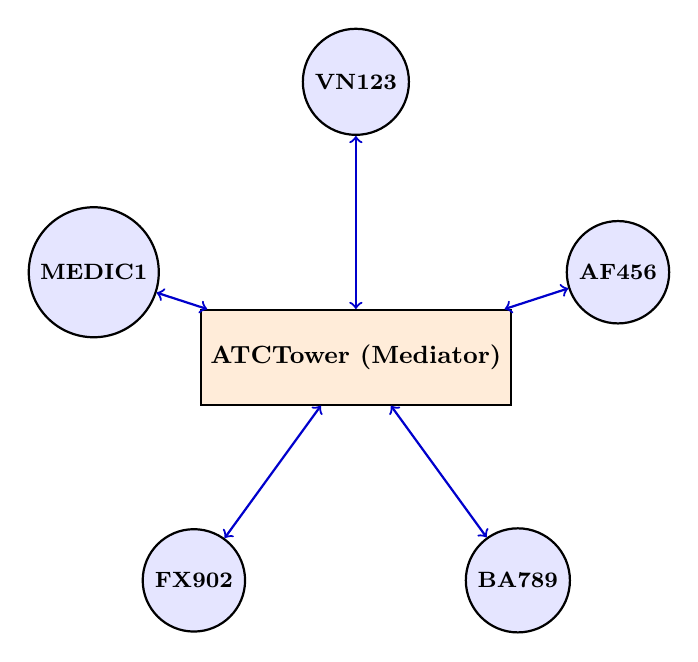
\begin{tikzpicture}[
    node/.style={circle, draw=black, thick, fill=blue!10, minimum size=1.3cm, font=\footnotesize\bfseries},
    mediator/.style={rectangle, draw=black, thick, fill=orange!15, minimum width=3.5cm, minimum height=1.2cm, font=\bfseries\small},
    conn/.style={<->, thick, blue!80!black}
]
\node[mediator] (ATC) at (0,0) {ATCTower (Mediator)};
\node[node] (A) at (90:3.5cm) {VN123};
\node[node] (B) at (18:3.5cm) {AF456};
\node[node] (C) at (306:3.5cm) {BA789};
\node[node] (D) at (234:3.5cm) {FX902};
\node[node] (E) at (162:3.5cm) {MEDIC1};

\draw[conn] (ATC) -- (A);
\draw[conn] (ATC) -- (B);
\draw[conn] (ATC) -- (C);
\draw[conn] (ATC) -- (D);
\draw[conn] (ATC) -- (E);
\end{tikzpicture}
}
\caption{Mediator Star Topology ($O(N)$ Links): Colleagues Communicate Solely Through the Central Hub}
\label{fig:star_topology}
\end{figure}

\subsection{Key Structural Components}
\begin{itemize}
    \item \textbf{Mediator Interface (\texttt{IATCMediator}):} Declares the protocol for communication with colleague objects (e.g., \texttt{requestLanding()}, \texttt{notifyRunwayClear()}, \texttt{broadcastEmergency()}).
    \item \textbf{Concrete Mediator (\texttt{ATCTower}):} Implements cooperative behavior by coordinating colleagues. It maintains the single source of truth for runway state, landing queues, and priority overrides.
    \item \textbf{Colleague Base Class (\texttt{Flight}):} Defines the abstract colleague entity. Each colleague maintains a reference to its mediator object rather than referencing peer colleagues.
    \item \textbf{Concrete Colleagues (\texttt{CommercialFlight}, \texttt{CargoFlight}, \texttt{EmergencyFlight}):} Implement specialized domain behavior. When an event occurs, colleagues notify their mediator instead of contacting other colleagues.
\end{itemize}

\newpage
\section{UML Class Diagrams}

\subsection{General GoF Mediator Pattern Structure}
The generic Mediator structure decouples colleague objects from one another by funneling all interaction logic through an abstract mediator interface.

\begin{figure}[htbp]
\centering
\resizebox{\linewidth}{!}{
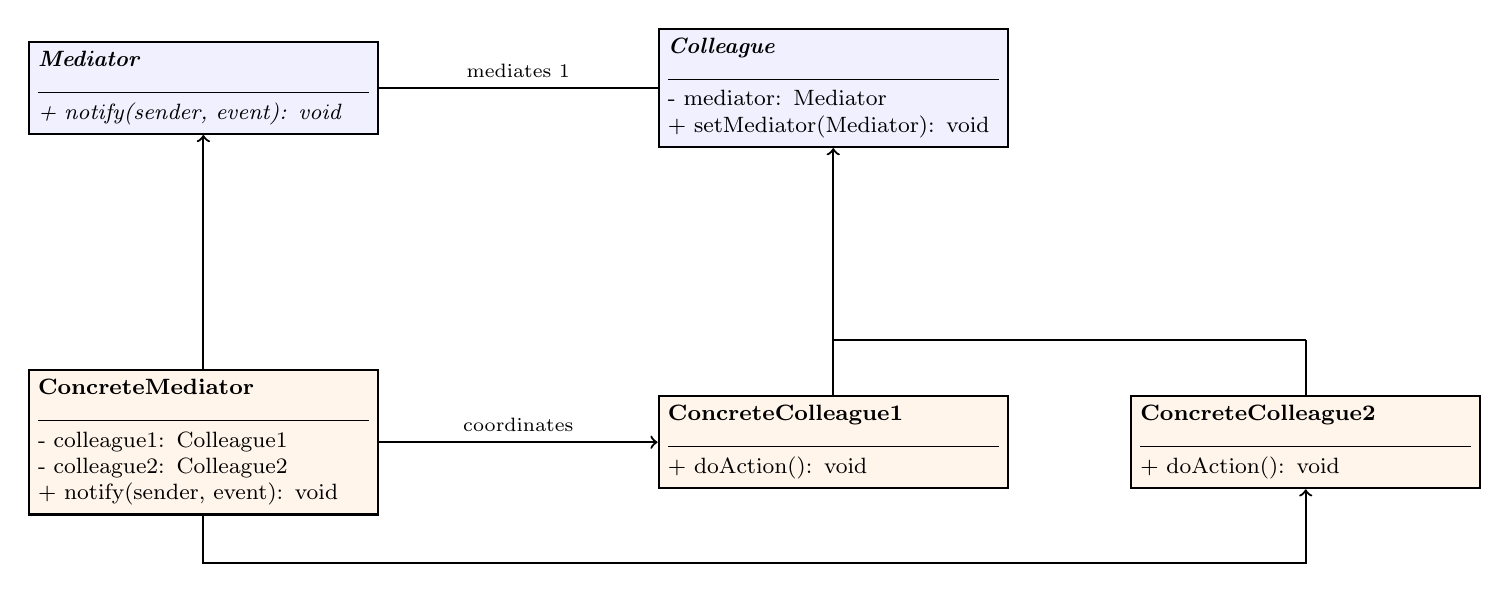
\begin{tikzpicture}[
    class/.style={rectangle, draw=black, thick, fill=white, text width=4.2cm, minimum height=1.1cm, font=\footnotesize},
    abstract/.style={class, fill=blue!6},
    concrete/.style={class, fill=orange!8}
]
% Top row: Mediator Interface (left) and Colleague Interface (right)
\node[abstract] (mediator) at (0, 0) {\textbf{\textit{Mediator}}\\\rule{4.2cm}{0.3pt}\\\textit{+ notify(sender, event): void}};
\node[abstract] (colleague) at (8, 0) {\textbf{\textit{Colleague}}\\\rule{4.2cm}{0.3pt}\\- mediator: Mediator\\+ setMediator(Mediator): void};

% Bottom row: spread out with absolute positioning, same Y level
\node[concrete] (concreteMediator) at (0, -4.5) {\textbf{ConcreteMediator}\\\rule{4.2cm}{0.3pt}\\- colleague1: Colleague1\\- colleague2: Colleague2\\+ notify(sender, event): void};
\node[concrete] (colleague1) at (8, -4.5) {\textbf{ConcreteColleague1}\\\rule{4.2cm}{0.3pt}\\+ doAction(): void};
\node[concrete] (colleague2) at (14, -4.5) {\textbf{ConcreteColleague2}\\\rule{4.2cm}{0.3pt}\\+ doAction(): void};

% Generalization arrows
\draw[->, thick] (concreteMediator.north) -- (mediator.south);
\draw[thick] (colleague1.north) -- ++(0,0.7) coordinate (cBusL);
\draw[thick] (colleague2.north) -- ++(0,0.7) coordinate (cBusR);
\draw[thick] (cBusL) -- (cBusR);
\draw[->, thick] (cBusL -| colleague.south) -- (colleague.south);

% Associations
\draw[thick] (colleague.west) -- (mediator.east) node[midway, above, font=\scriptsize] {mediates 1};

% Coordinate lines from ConcreteMediator to ConcreteColleagues
% To Colleague1: straight line
\draw[->, thick] (concreteMediator.east) -- (colleague1.west) node[midway, above, font=\scriptsize] {coordinates};
% To Colleague2: route under Colleague1 to avoid crossing
\draw[->, thick] (concreteMediator.south) -- ++(0,-0.6) -| (colleague2.south);
\end{tikzpicture}
}
\caption{General GoF Mediator Pattern UML Structure}
\label{fig:general_mediator_uml}
\end{figure}

\subsection{Airport Air Traffic Control Mediator Class Hierarchy}
For our ATC runway coordination engine, \texttt{ATCTower} serves as the central mediator managing flight registrations, holding queues, and landing clearances across specialized flight colleagues.

\begin{figure}[htbp]
\centering
\resizebox{\linewidth}{!}{
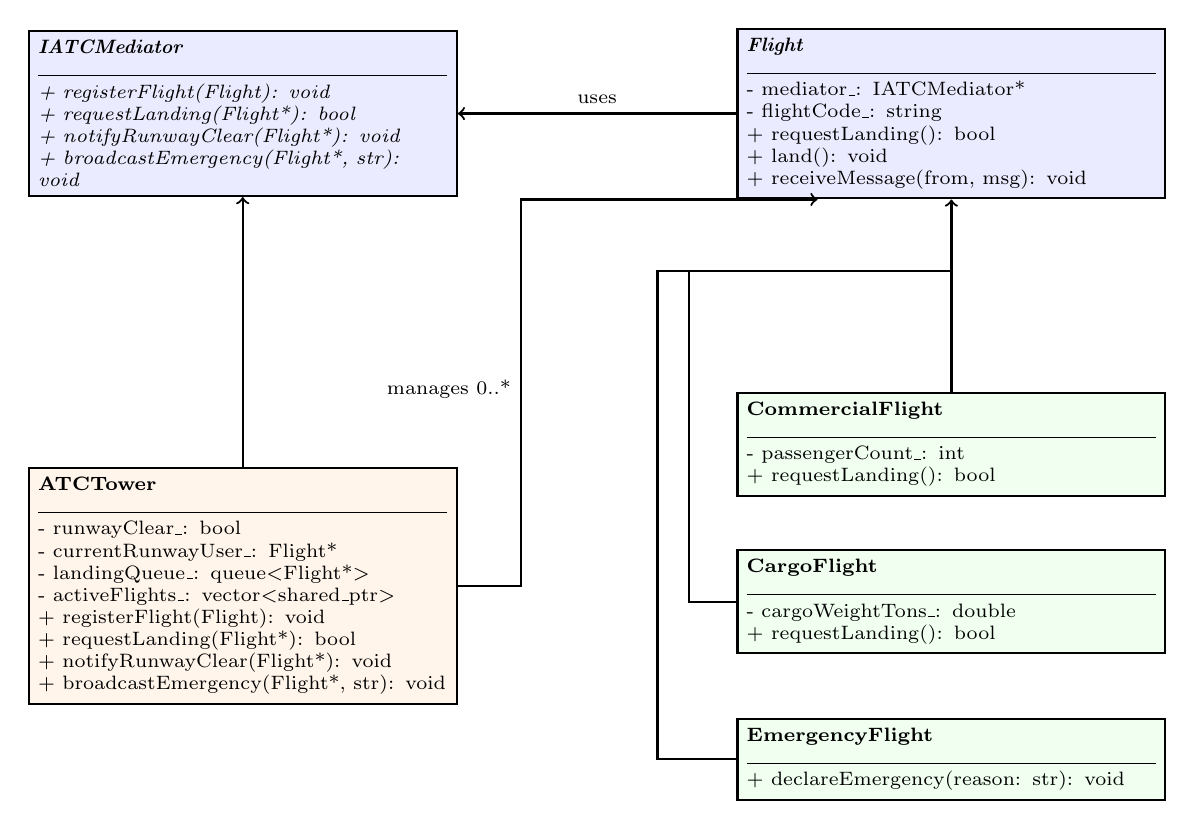
\begin{tikzpicture}[
    class/.style={rectangle, draw=black, thick, fill=white, text width=5.2cm, font=\scriptsize},
    abstract/.style={class, fill=blue!8},
    medclass/.style={class, fill=orange!8},
    colclass/.style={class, fill=green!6}
]
% Top row: Mediator Interface (left) and Flight Base Class (right)
\node[abstract] (iMediator) at (0, 0) {\textbf{\textit{IATCMediator}}\\\rule{5.2cm}{0.3pt}\\\textit{+ registerFlight(Flight): void}\\\textit{+ requestLanding(Flight*): bool}\\\textit{+ notifyRunwayClear(Flight*): void}\\\textit{+ broadcastEmergency(Flight*, str): void}};

\node[abstract] (flightBase) at (9, 0) {\textbf{\textit{Flight}}\\\rule{5.2cm}{0.3pt}\\- mediator\_: IATCMediator*\\- flightCode\_: string\\+ requestLanding(): bool\\+ land(): void\\+ receiveMessage(from, msg): void};

% Bottom-left: Concrete Mediator
\node[medclass] (atcTower) at (0, -6) {\textbf{ATCTower}\\\rule{5.2cm}{0.3pt}\\- runwayClear\_: bool\\- currentRunwayUser\_: Flight*\\- landingQueue\_: queue$<$Flight*$>$\\- activeFlights\_: vector$<$shared\_ptr$>$\\+ registerFlight(Flight): void\\+ requestLanding(Flight*): bool\\+ notifyRunwayClear(Flight*): void\\+ broadcastEmergency(Flight*, str): void};

% Bottom-right column: Concrete Colleagues (stacked vertically)
\node[colclass] (commFlight) at (9, -4.2) {\textbf{CommercialFlight}\\\rule{5.2cm}{0.3pt}\\- passengerCount\_: int\\+ requestLanding(): bool};

\node[colclass] (cargoFlight) at (9, -6.2) {\textbf{CargoFlight}\\\rule{5.2cm}{0.3pt}\\- cargoWeightTons\_: double\\+ requestLanding(): bool};

\node[colclass] (emergFlight) at (9, -8.2) {\textbf{EmergencyFlight}\\\rule{5.2cm}{0.3pt}\\+ declareEmergency(reason: str): void};

% Inheritance: ATCTower -> IATCMediator
\draw[->, thick] (atcTower.north) -- (iMediator.south);

% Association: Flight uses IATCMediator
\draw[->, thick] (flightBase.west) -- (iMediator.east) node[midway, above, font=\scriptsize] {uses};

% Association: ATCTower manages Flight (routed explicitly, entering Flight's south
% edge well clear of both the "uses" association and the colleague-inheritance trunk)
\coordinate (flightManageAnchor) at ([xshift=-1.7cm]flightBase.south);
\draw[->, thick] (atcTower.east) -- ++(0.8,0) coordinate (M1) |- (flightManageAnchor);
\node[font=\scriptsize, anchor=east] at ([yshift=2.5cm]M1) {manages 0..*};

% Colleague inheritance: Unified tree via a bus at y=-2.0
\draw[->, thick] (commFlight.north) -- (flightBase.south);
% Route CargoFlight into the trunk
\draw[thick] (cargoFlight.west) -- ++(-0.6,0) coordinate (C1) -- (C1 |- 0,-2.0) -- (9,-2.0);
% Route EmergencyFlight into the trunk
\draw[thick] (emergFlight.west) -- ++(-1.0,0) coordinate (E1) -- (E1 |- 0,-2.0) -- (9,-2.0);
\end{tikzpicture}
}
\caption{Airport Air Traffic Control Mediator Class Hierarchy}
\label{fig:atc_mediator_uml}
\end{figure}

\newpage
\section{Pattern-Based Implementation in C++17}

\subsection{Architectural Design Rationale: Memory Management \& Queuing}
In our C++17 implementation:
\begin{itemize}
    \item \textbf{Ownership Topology:} \texttt{ATCTower} maintains ownership of active airspace participants using \texttt{std::vector<std::shared\_ptr<Flight>>}. Colleague instances store a non-owning raw pointer (\texttt{IATCMediator*}) to the mediator to prevent reference cycles.
    \item \textbf{FIFO Holding Pattern Queue:} When the runway is occupied, arriving flights are pushed to a \texttt{std::queue<Flight*> landingQueue\_}.
    \item \textbf{Automatic Cascade on Vacation:} When the current runway user invokes \texttt{notifyRunwayClear()}, the tower automatically pops the next flight from the queue, grants clearance, and triggers its landing sequence.
    \item \textbf{Emergency Priority Overrides:} When an \texttt{EmergencyFlight} calls its \texttt{declareEmergency()} method, standard traffic is alerted. The emergency flight is then granted immediate runway access.
\end{itemize}

\subsection{Source Code Implementation}
The following listings demonstrate the complete, warning-free implementation (\texttt{Mediator/src/pattern.cpp}).

\begin{lstlisting}[caption={Mediator Interface and Flight Colleague Base Class}]
namespace pattern {

class Flight; // Forward declaration

// Abstract Mediator Interface
class IATCMediator {
public:
    virtual ~IATCMediator() = default;
    virtual void registerFlight(std::shared_ptr<Flight> flight) = 0;
    virtual bool requestLanding(Flight* flight) = 0;
    virtual void notifyRunwayClear(Flight* flight) = 0;
    virtual void broadcastEmergency(Flight* flight, const std::string& reason) = 0;
};

// Colleague Base Class
class Flight {
protected:
    IATCMediator* mediator_;
    std::string flightCode_;

public:
    Flight(std::string code, IATCMediator* mediator)
        : mediator_(mediator), flightCode_(std::move(code)) {}
    virtual ~Flight() = default;

    const std::string& getCode() const { return flightCode_; }

    virtual bool requestLanding() {
        std::cout << "[" << flightCode_ << "] Requesting landing clearance from ATC Tower...\n";
        return mediator_->requestLanding(this);
    }

    virtual void land() {
        std::cout << "[" << flightCode_ << "] >>> TOUCHDOWN SUCCESSFUL on Runway 07L. Clearing runway...\n";
        mediator_->notifyRunwayClear(this);
    }

    virtual void receiveMessage(const std::string& from, const std::string& msg) {
        std::cout << "  [" << flightCode_ << " Radio] Received from " << from << ": " << msg << "\n";
    }
};
\end{lstlisting}

\newpage
\begin{lstlisting}[caption={Concrete Colleagues: Commercial, Cargo, and Emergency Flights}]
// Concrete Colleague: Commercial Passenger Flight
class CommercialFlight : public Flight {
private:
    int passengerCount_;

public:
    CommercialFlight(std::string code, int passengers, IATCMediator* mediator)
        : Flight(std::move(code), mediator), passengerCount_(passengers) {}

    bool requestLanding() override {
        std::cout << "[" << flightCode_ << " (Commercial - " << passengerCount_ << " passengers)] "
                  << "Approaching airport. Requesting landing clearance...\n";
        return mediator_->requestLanding(this);
    }
};

// Concrete Colleague: Cargo Freight Flight
class CargoFlight : public Flight {
private:
    double cargoWeightTons_;

public:
    CargoFlight(std::string code, double cargoTons, IATCMediator* mediator)
        : Flight(std::move(code), mediator), cargoWeightTons_(cargoTons) {}

    bool requestLanding() override {
        std::cout << "[" << flightCode_ << " (Cargo - " << cargoWeightTons_ << " tons)] "
                  << "Heavy transport on final approach. Requesting landing clearance...\n";
        return mediator_->requestLanding(this);
    }
};

// Concrete Colleague: Emergency Flight (Air Ambulance / Medevac)
class EmergencyFlight : public Flight {
public:
    using Flight::Flight;

    void declareEmergency(const std::string& reason) {
        std::cout << "\n[" << flightCode_ << " (EMERGENCY)] !!! MAYDAY MAYDAY MAYDAY: " << reason << " !!!\n";
        mediator_->broadcastEmergency(this, reason);
    }
};
\end{lstlisting}

\newpage
\begin{lstlisting}[caption={Concrete Mediator: Central ATCTower Engine}]
// Concrete Mediator: Air Traffic Control Tower
class ATCTower : public IATCMediator {
private:
    bool runwayClear_ = true;
    Flight* currentRunwayUser_ = nullptr;
    std::queue<Flight*> landingQueue_;
    std::vector<std::shared_ptr<Flight>> activeAirspaceFlights_;

public:
    void registerFlight(std::shared_ptr<Flight> flight) override {
        activeAirspaceFlights_.push_back(flight);
        std::cout << "[ATC Tower] Radar tracked: Flight " << flight->getCode() 
                  << " entered airspace and registered with tower.\n";
    }

    bool requestLanding(Flight* flight) override {
        if (runwayClear_) {
            runwayClear_ = false;
            currentRunwayUser_ = flight;
            std::cout << "[ATC Tower] Clearance GRANTED for " << flight->getCode() 
                      << ". Runway 07L is CLEAR for landing.\n";
            return true;
        } else {
            landingQueue_.push(flight);
            std::cout << "[ATC Tower] HOLDING PATTERN for " << flight->getCode() 
                      << ". Runway 07L currently OCCUPIED by " << currentRunwayUser_->getCode() 
                      << ". Added to queue (Queue position: " << landingQueue_.size() << ").\n";
            return false;
        }
    }

    void notifyRunwayClear(Flight* flight) override {
        if (currentRunwayUser_ == flight) {
            std::cout << "[ATC Tower] Runway 07L VACATED by " << flight->getCode() << ".\n";
            currentRunwayUser_ = nullptr;
            runwayClear_ = true;

            // Automatically dispatch the next flight waiting in queue
            if (!landingQueue_.empty()) {
                Flight* nextFlight = landingQueue_.front();
                landingQueue_.pop();
                std::cout << "[ATC Tower] Calling next queued flight: Clearance GRANTED for " 
                          << nextFlight->getCode() << ".\n";
                runwayClear_ = false;
                currentRunwayUser_ = nextFlight;
                nextFlight->land();
            } else {
                std::cout << "[ATC Tower] Runway 07L is currently IDLE and ready for traffic.\n";
            }
        }
    }

    void broadcastEmergency(Flight* emergencyFlight, const std::string& reason) override {
        std::cout << "[ATC Tower ALERT] Priority Emergency declared by " << emergencyFlight->getCode() 
                  << " (" << reason << "). Cleared for IMMEDIATE priority landing!\n";
        
        // Broadcast safety alert to all other flights in airspace
        for (const auto& f : activeAirspaceFlights_) {
            if (f.get() != emergencyFlight) {
                f->receiveMessage("ATC Tower", "AIRSPACE ADVISORY: Yield runway for emergency flight " 
                                  + emergencyFlight->getCode() + " (" + reason + ").");
            }
        }

        // Fast-track emergency landing
        runwayClear_ = false;
        currentRunwayUser_ = emergencyFlight;
        emergencyFlight->land();
    }
};

} // namespace pattern
\end{lstlisting}

\newpage
\subsection{Execution Walkthrough \& Step-by-Step Simulation Trace}

Table~\ref{tab:mediator_execution_trace} summarizes the lifecycle events, runway states, and automatic queue dispatches during simulation:

\begin{table}[htbp]
\centering
\small
\resizebox{\linewidth}{!}{
\begin{tabular}{c p{3.8cm} c p{2.2cm} p{5.0cm}}
\toprule
\textbf{Step} & \textbf{Event / Trigger} & \textbf{Runway} & \textbf{Holding Queue} & \textbf{ATC Tower Action / Dispatched Output} \\
\midrule
1 & Radar Registration & CLEAR & Empty & \texttt{VN123}, \texttt{FX902}, \texttt{BA789} registered with central radar. \\
\addlinespace
2 & \texttt{VN123} Landing Req & OCCUPIED & Empty & Runway 07L is free; clearance granted to \texttt{VN123}. \\
\addlinespace
3 & \texttt{FX902} Landing Req & OCCUPIED & [\texttt{FX902}] & Runway occupied by \texttt{VN123}; \texttt{FX902} pushed to queue position 1. \\
\addlinespace
4 & \texttt{BA789} Landing Req & OCCUPIED & [\texttt{FX902}, \texttt{BA789}] & Runway occupied; \texttt{BA789} pushed to queue position 2. \\
\addlinespace
5 & \texttt{VN123} Vacates & OCCUPIED & [\texttt{BA789}] & Tower detects vacancy, pops \texttt{FX902}, and clears \texttt{FX902} for landing. \\
\addlinespace
6 & \texttt{FX902} Vacates & OCCUPIED & Empty & Tower detects vacancy, pops \texttt{BA789}, and clears \texttt{BA789} for landing. \\
\addlinespace
7 & \texttt{BA789} Vacates & CLEAR & Empty & \texttt{BA789} vacates runway; runway status transitions to IDLE. \\
\addlinespace
8 & \texttt{MEDIC1} Mayday & OCCUPIED & Standard Halted & Tower broadcasts advisory to all aircraft; \texttt{MEDIC1} lands with immediate priority. \\
\bottomrule
\end{tabular}
}
\caption{Dynamic Execution and Queue Cascade Trace in the Mediator System}
\label{tab:mediator_execution_trace}
\end{table}

\newpage
\section{Evaluation of Trade-offs}

\subsection{Advantages}
\begin{itemize}
    \item \textbf{Decoupled Colleagues ($O(N)$ vs. $O(N^2)$ Complexity):} Colleagues no longer reference peers. Flights communicate exclusively with \texttt{IATCMediator}, drastically reducing class inter-dependencies.
    \item \textbf{Centralized Control \& Business Logic (SRP Compliance):} Runway assignment policies, separation standards, and holding pattern queues are centralized in \texttt{ATCTower}, freeing colleague classes to focus solely on flight mechanics.
    \item \textbf{High Extensibility (OCP Compliance):} New flight categories (e.g., \texttt{Helicopter}, \texttt{AutonomousDroneDelivery}) can be introduced without modifying existing flight implementations.
    \item \textbf{Elimination of Dangling Pointers:} When an aircraft lands and exits the airspace, it unregisters from the central mediator in $O(1)$ time with zero ripple effects across other flight objects.
\end{itemize}

\subsection{Disadvantages and Limitations}
\begin{itemize}
    \item \textbf{"God Object" Anti-Pattern Risk:} As a system evolves, business rules, filtering policies, and coordination protocols can cause the ConcreteMediator to become monolithic, overly complex, and difficult to maintain.
    \item \textbf{Single Point of Failure / Bottleneck:} If the mediator crashes or experiences thread lockups, communication between all colleagues ceases entirely.
    \item \textbf{Indirection Overhead:} Direct method calls between colleagues are replaced with virtual function dispatch through the mediator, adding a minor layer of runtime indirection.
\end{itemize}

\section{Applications}

The Mediator pattern is widely used in modern software engineering to manage complex interaction flows:

\begin{itemize}
    \item \textbf{ASP.NET Core MediatR Library:} In enterprise CQRS (Command Query Responsibility Segregation) web applications, MediatR acts as an in-process mediator. Web API controllers send Command or Query objects to MediatR without knowing which handler processes the request. Cross-cutting pipeline behaviors (such as logging, validation, metrics, and transaction management) are attached centrally to the mediator pipeline.
    \item \textbf{iOS Coordinator Pattern:} In iOS Swift development, the Coordinator pattern decouples UI ViewControllers from navigation logic. Instead of ViewController A instantiating and pushing ViewController B directly, ViewControllers notify a central \texttt{Coordinator}, which manages navigation transitions and deep linking.
    \item \textbf{GUI Dialog and Form Controllers:} Complex dialog windows (containing text boxes, checkboxes, sliders, and submit buttons) use a Form Mediator. When a user checks a box, the form mediator automatically enables, disables, or validates dependent fields without individual UI widgets referencing each other.
    \item \textbf{Real-Time Chat and Collaboration Gateways:} WebSocket servers function as mediators, managing room subscriptions, message formatting, and routing between active chat clients.
    \item \textbf{Microservices Orchestration and Saga Coordinators:} In distributed transaction management, an orchestrator service coordinates the sequence of steps across independent microservices (e.g., payment, inventory, shipping) without those services communicating with each other directly. The orchestrator issues commands, tracks completion state, and triggers compensating transactions on failure, centralizing business transaction logic instead of scattering it across a peer-to-peer choreography.
\end{itemize}

\newpage
\section{Observer and Interpreter Integration}

In production-grade software architectures, the Mediator pattern frequently pairs with the Observer and Interpreter patterns:

\subsection{Combining Mediator with the Observer Pattern (Event Aggregator)}
While a standard Mediator pattern uses direct method invocations on colleague references, pairing it with the Observer pattern creates an \textbf{Event Aggregator / Event Bus}.

Colleague components register as observers with a central \texttt{EventMediator}. When an event occurs, the publishing colleague dispatches an event object to the Mediator without holding any reference to subscribers. The Mediator routes the payload to registered subscriber observers based on event types. This combines the unidirectional loose coupling of Observer with the centralized topology of Mediator.

\subsection{Combining Mediator with the Interpreter Pattern}
In dynamic, rule-driven systems—such as airport slot allocation engines, automated trade routing, or access control gateways—the Mediator's internal coordination rules should not be hardcoded into C++ source code.

Instead, the central \texttt{Mediator} embeds an \textbf{AST Interpreter}. When colleagues submit requests (e.g., flight landing requests with parameters such as fuel level, aircraft weight, and passenger count), the Mediator interprets dynamic domain-specific expressions (e.g., \texttt{"(fuel < 10\%) OR (patient == CRITICAL)"}) at runtime to compute queue priority dynamically without requiring recompilation.

\section{Conclusion}

The Mediator Design Pattern provides an indispensable architectural solution for untangling complex, many-to-many component interactions. By replacing direct peer-to-peer dependencies with a centralized coordinator, the pattern eliminates $O(N^2)$ mesh complexity and establishes strict compliance with the Single Responsibility and Open-Closed Principles.

Through our C++17 implementation of the Airport Air Traffic Control simulation, we demonstrated how centralizing runway state machines, holding pattern queues, and emergency Mayday overrides in \texttt{ATCTower} allows specialized flight colleagues (\texttt{CommercialFlight}, \texttt{CargoFlight}, \texttt{EmergencyFlight}) to operate in total isolation from one another. When integrated with smart pointer lifetime management and combined with the Observer and Interpreter patterns, the Mediator pattern provides a robust, extensible foundation for real-world enterprise web backends, mobile UI coordinators, and real-time distributed systems.

\newpage
\section*{References}
\addcontentsline{toc}{section}{References}
\begin{itemize}
    \item Gamma, E., Helm, R., Johnson, R., \& Vlissides, J. (1994). \textit{Design Patterns: Elements of Reusable Object-Oriented Software}. Addison-Wesley.
    \item Buschmann, F., Meunier, R., Rohnert, H., Sommerlad, P., \& Stal, M. (1996). \textit{Pattern-Oriented Software Architecture: A System of Patterns} (Vol. 1). John Wiley \& Sons.
    \item Fowler, M. (2002). \textit{Patterns of Enterprise Application Architecture}. Addison-Wesley.
    \item Meyers, S. (2014). \textit{Effective Modern C++: 42 Specific Ways to Improve Your Use of C++11 and C++14}. O'Reilly Media.
    \item Bogard, J. (2015). \textit{MediatR: Simple, unambitious mediator implementation in .NET}. \url{https://github.com/jbogard/MediatR}
    \item Klishevich, S. (2015). \textit{The Coordinator Pattern in iOS Architecture}. \url{https://khanlou.com/2015/01/the-coordinator/}
    \item Refactoring.Guru. (2024). \textit{Design Patterns: Mediator Pattern}. \url{https://refactoring.guru/design-patterns/mediator}
\end{itemize}

\end{document}

